% !TEX root = ../../phdthesis_tawatr.tex 
\newcommand{\gtes}{(\gainp,\twistp,\shearp,\splittingp)}
\renewcommand{\thisdir}{_content/reg1d_synthetic_1d}
\renewcommand{\figdir}{\thisdir/_fig}
\chapter[Synthetic Experiments and Discussion]{Synthetic experiments and Discussion}
\label{chap:synthetic}

In this chapter, we test the proposed methods (as described in Chapter \ref{chap:method}) using the average ssq impedance to estimate the regional mean 1D conductivity profile and deriving galvanic distortion-related indicators through synthetic examples. 
%
Synthetic 1D and 3D models are used, and the galvanic distortion was simulated with the random distortion parameters -- $\gainp, \twistp, \shearp$ and $\splittingp$. 
%
As we introduce the theoretical model of regional mean 1D conductivity profile (Eqs. \ref{eq:regional_mean_linear} and \ref{eq:regional_mean_log}), we examined if it is consistent with the model of regional mean 1D conductivity profile estimated from the average ssq impedance. 

\section[1D examples]{Estimating a model of regional mean 1D profile: 1D example}\label{sect:example_1d}

%\begin{itemize}
%	\item 
	In this work, the synthetic layered-Earth model (Figure \ref{fig:lyrearth_model}) was made based on \citet{jones1999a}, which has the main feature of resistive upper crust (3.5--14.8 km depth) and conductive lower crust (14.8--33.3 km depth). This feature is commonly found in the continental crust \citep{jones1999a}.
%	\item 
	The corresponding MT response was calculated in the period range of (Figure \ref{fig:lyrearth_resp}) using the analytic solution \citep{constable1987a}.
%	\item 
	The heterogeneity embedded in the lower crust layer is detectable in this period range, while any structures confined in the near-surface layer -- a few kilometers or less, which is shallower and thinner than the inductive scale length of interest -- are considered to be the galvanic distorters.
%\end{itemize}

%% ==== Figure: The layer earth model
	\begin{figure}[t]
		\centering
		\subfigure[]{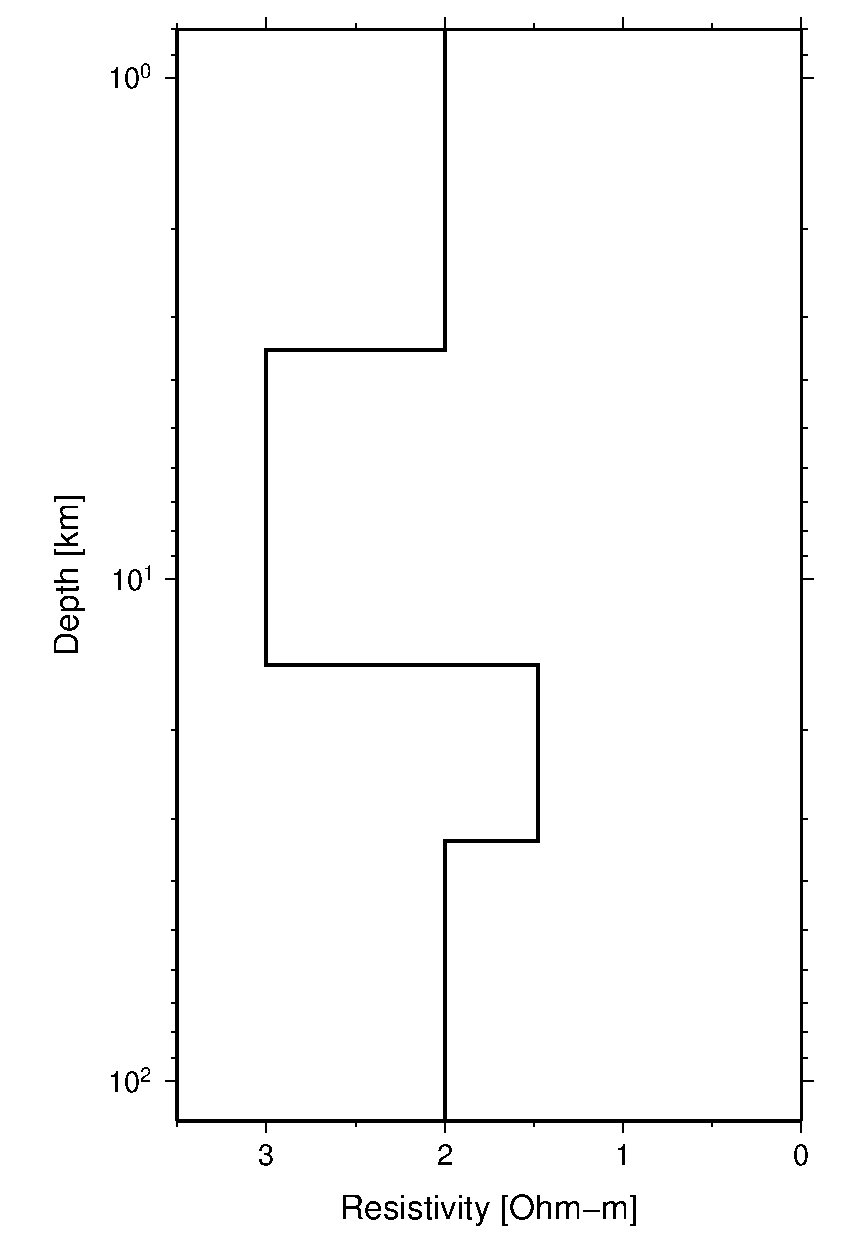
\includegraphics[scale=\plotinvmodelscale]{\figdir/model_lyr11a_cropped.pdf}
		\label{fig:lyrearth_model}
		}
		\subfigure[]{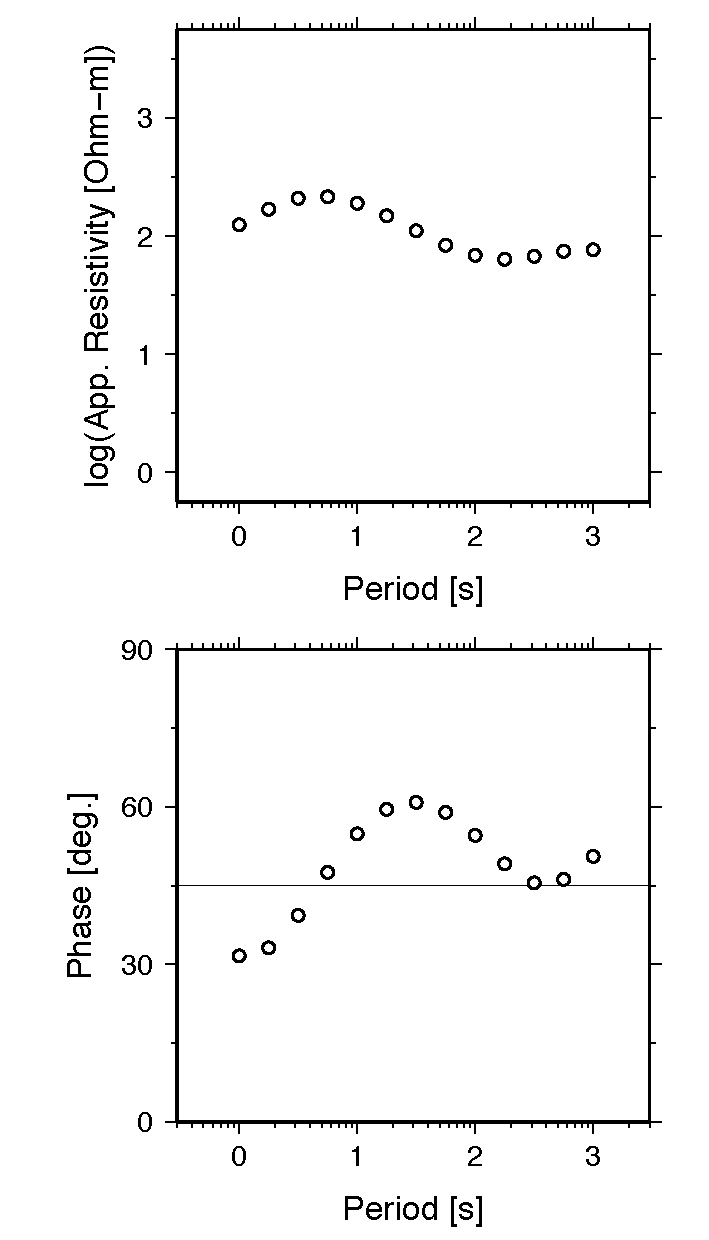
\includegraphics[scale=\plotmtrespscale]{\figdir/mesh-m01a-lyr11a_mt_arsphs_inv.pdf}
		\label{fig:lyrearth_resp}
		}
		\caption[Layered-earth model used in this study and corresponding response]{\subref{fig:lyrearth_model} Layered-Earth model used in this work. \subref{fig:lyrearth_resp} Corresponding MT response (apparent resistivity and phase).}\label{fig:lyrearth_resp}
	\end{figure}

%\begin{itemize}
%	\item 
	As described earlier, the near-surface distorters cause spatial aliasing in the data.
%	\item 
	The distortion parameters in the Groom--Bailey framework -- site gain $\gainp$, twist $\twistp$, shear $\shearp$ and splitting $\splittingp$ parameters -- can reasonably be assumed to be random \citep[e.g.,][]{avdeeva2015a}. 
%	\item 
	Given that the MT array consists of 25 MT stations in our synthetic tests, 25 sets of real-valued parameters $\gtes$ are generated from the normal distribution.
	Also, to quantify the galvanic distortion strength, the standard deviation (SD) used in the normal distribution ranges from 0.1--0.5 (Figure \ref{fig:dparam}). Note that when the SD was greater than 0.3, the randomly generated numbers were less likely to comply with the theoretical normal distribution, and more like the uniform distribution.
	We further assume that each set of distortion parameters has the mean of zero and is within $(-1,+1)$. Note that the random site gain was made in an logarithmic scale.
	Eventually, we have five MT datasets, 25 stations each, distorted with different galvanic distortion strength. The distorted impedances are calculated using Eq. \eqref{eq:z_distorted} by applying these random parameters to the 1D impedance (as shown in Figure \ref{fig:lyrearth_resp}).
%\end{itemize}

%%% ==== Figure: Distortion parameter plot and its distribution
	\begin{figure}[t]	
		\centering
		\subfigure[]{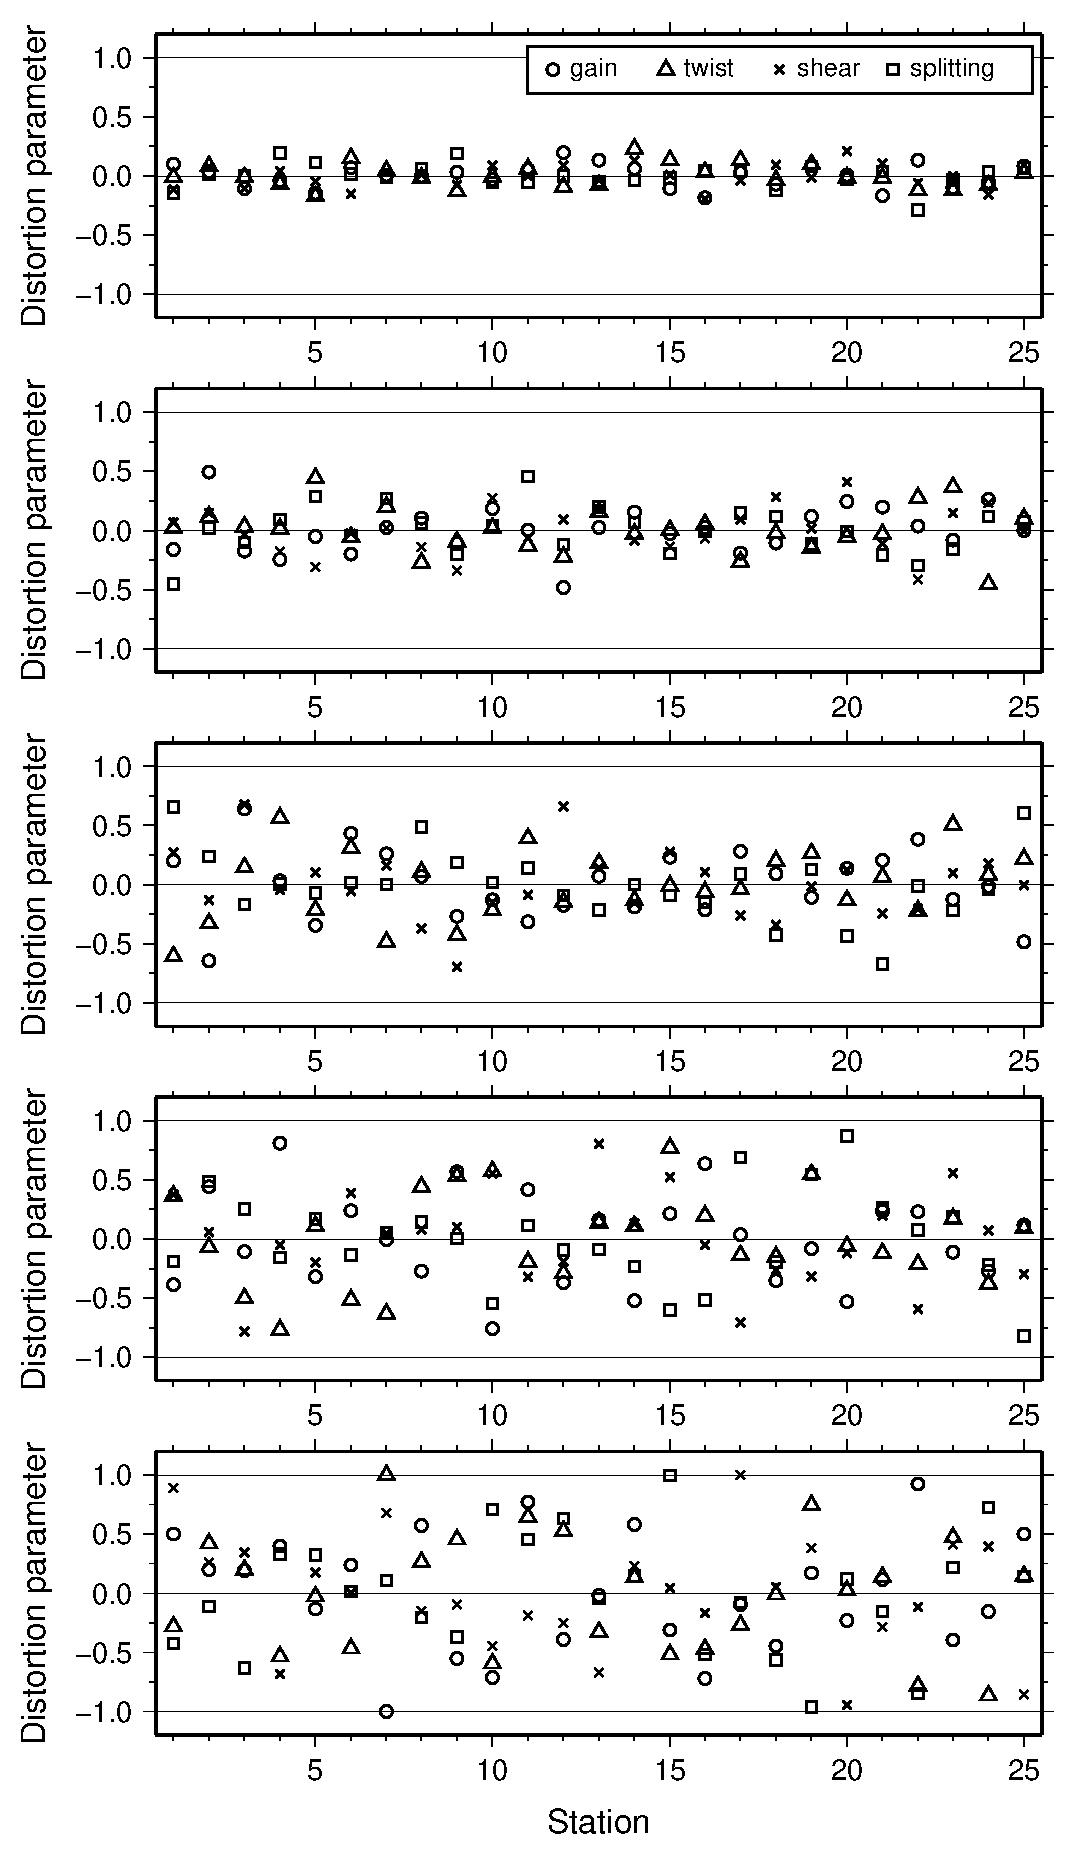
\includegraphics[scale=0.3]{\figdir/gtes.pdf}
		\label{fig:dparam_value}
		}
		\subfigure[]{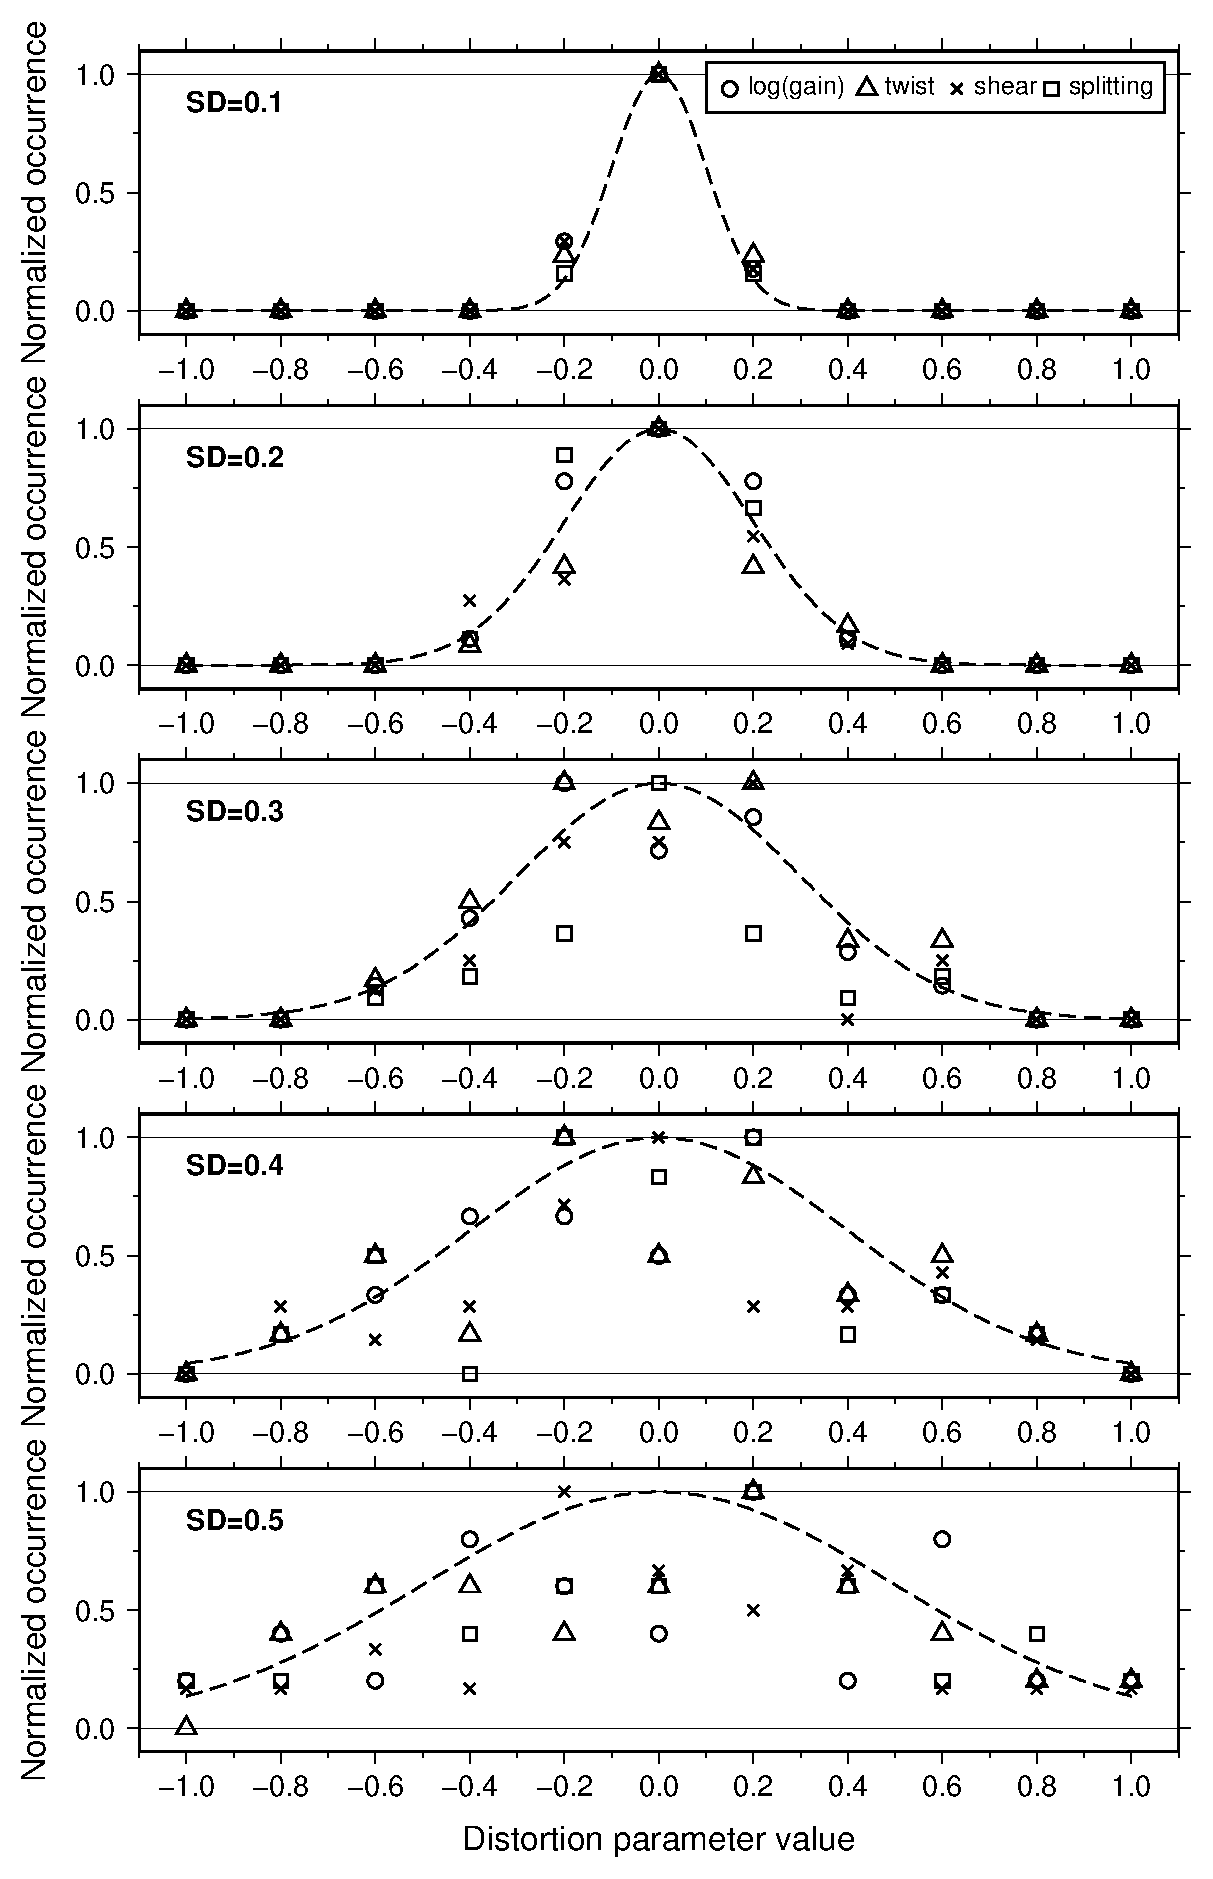
\includegraphics[scale=0.3]{\figdir/gtes_hist2.pdf}
		\label{fig:dparam_hist}
		}
		\caption[Distortion parameters and their distribution]{\subref{fig:dparam_value} Random distortion parameter values generated from the normal distribution with different SDs. \subref{fig:dparam_hist} Distribution of the distortion parameters. The normalized occurrence is the number of occurrences divided by the maximum number of occurrences at a single parameter value. Each distribution is compared with the probability density function of the theoretical normal distribution for the given SD (dashed lines).}
		\label{fig:dparam}
	\end{figure}
	
%% ==== Results: Individual
% \red{-- Individual --}
 
%\begin{itemize}
%	\item 
	In the 1D Earth, the galvanic distortion causes no phase mixing, but only a static shift in magnitude of the MT components (Figure \ref{fig:resp1d_example_distorted_zij}), whereas the galvanic distortion, as proven, only causes the static shift in the rotationally invariant impedances (Figure \ref{fig:resp1d_example_distorted_zinv}). The MT data in this example is distorted with $\gtes$ of $(1.20,0.11,-0.37,0.49)$.
%	\red{Note that the $xx$ phase  }
%	\item 
%	The example of data in Figure \ref{fig:resp1d_example_distorted} distorted with $\gtes=(1.20,0.11,-0.37,0.49)$ . 
	In this example, the synthetic site gain $\gainp$ is greater than unity. Therefore the ssq impedance is shifed upward. As described in Section \ref{sect:distorted_invariants}, the site gain provides the same effect on the det and ssq impedances. Hence the det impedance is also supposed to be shifted upward, but here it is biased downward due to the shear and splitting parameters so that its magnitude is less than the undistorted impedance. 
%	\item 


	
		
%% ====	
	As the distortion parameters are randomly generated, the rotational invariant impedances are irregularly shifted (Figure \ref{fig:resp1d_individual_all_distorted_sd3a}), which resembles the results in \citet{berdichevsky1980a} (Figure \ref{fig:berdichevsky_result}). 
%	\item 
	The shift in the ssq impedance is solely due to the site gain, but the shift in the det impedance also includes the shear and splitting parameters. 
	As mentioned, this behaviour could be problematic because the effect of the shear and splitting parameters and the site gain is indistinguishable, if the det impedance is chosen.
%\end{itemize}



%% ==== Results: Average
% \red{-- Average --}
 
%\begin{itemize}
%	\item
	To examine the effect of galvanic distortion strength on the regional mean impedance, the average det and ssq impedances for each distorted dataset (Figure \ref{fig:resp1d_avg_distorted}) were calculated using Eqs. \eqref{eq:zdet_mean} and \eqref{eq:zssq_mean}, respectively. Here, the error bar is the standard deviation of the data and therefore represents the level of dispersion of the sounding curves. The large error bars correspond to strong galvanic distortion strengths. For example, the dataset distorted with an SD of 0.5 has the largest error bar. 
%	\item 
	At the same strength of galvanic distortion, the average det impedances appear to be more dispersed than the average ssq impedances, because the shear and splitting parameters also affect the det impedance. 
%	\item 
	From the results, the average det impedance is biased downward by the galvanic distortion, although its effect is not noticeable when the SD of the distortion parameters is less than 0.2.
	On the contrary, the average ssq impedances remain the same at all galvanic distortion strengths.
	This is consistent with the theoretical derivation that the average ssq impedance would give the unbiased approximation of the model of the regional mean 1D conductivity profile \citep{rung-arunwan2016a}.
%\end{itemize}

%%% ==== Figure: Distored 1D response example
	\begin{figure}[t]
		\centering
		\subfigure[]{
		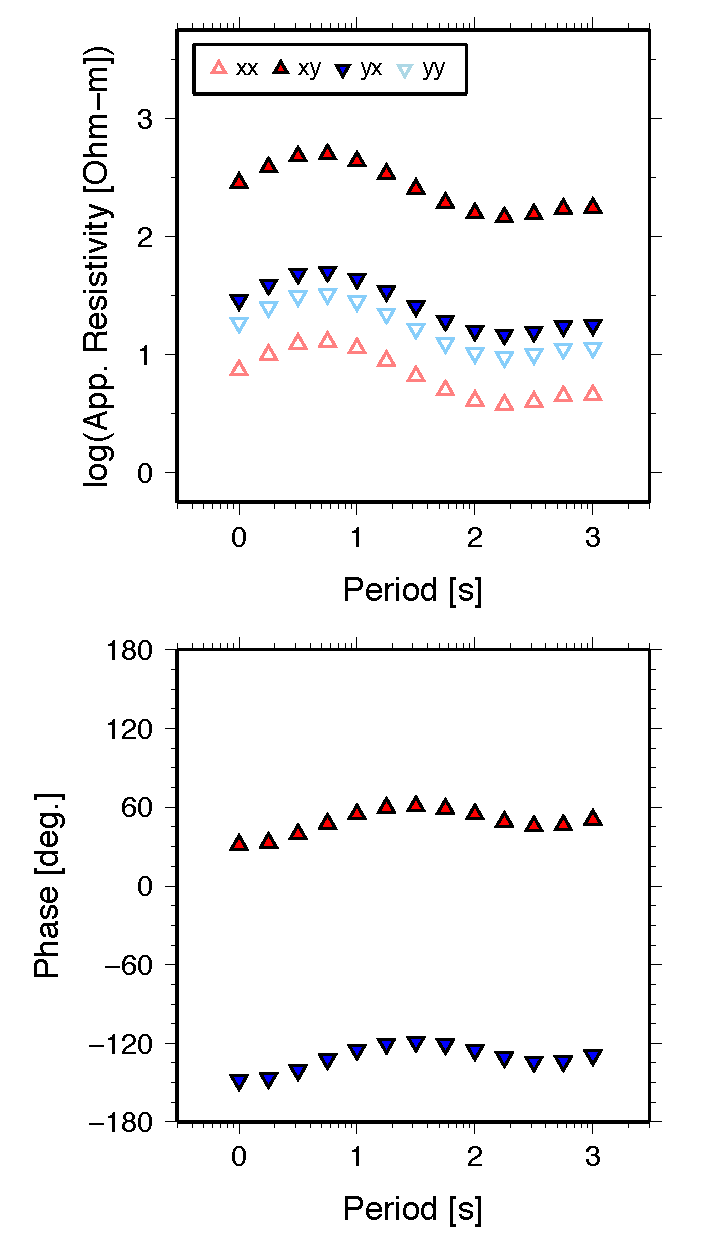
\includegraphics[scale=\plotmtrespscale]{\figdir/lyr11a_syn0203_mt_arsphs.pdf}
		\label{fig:resp1d_example_distorted_zij}
		}
		\subfigure[]{
		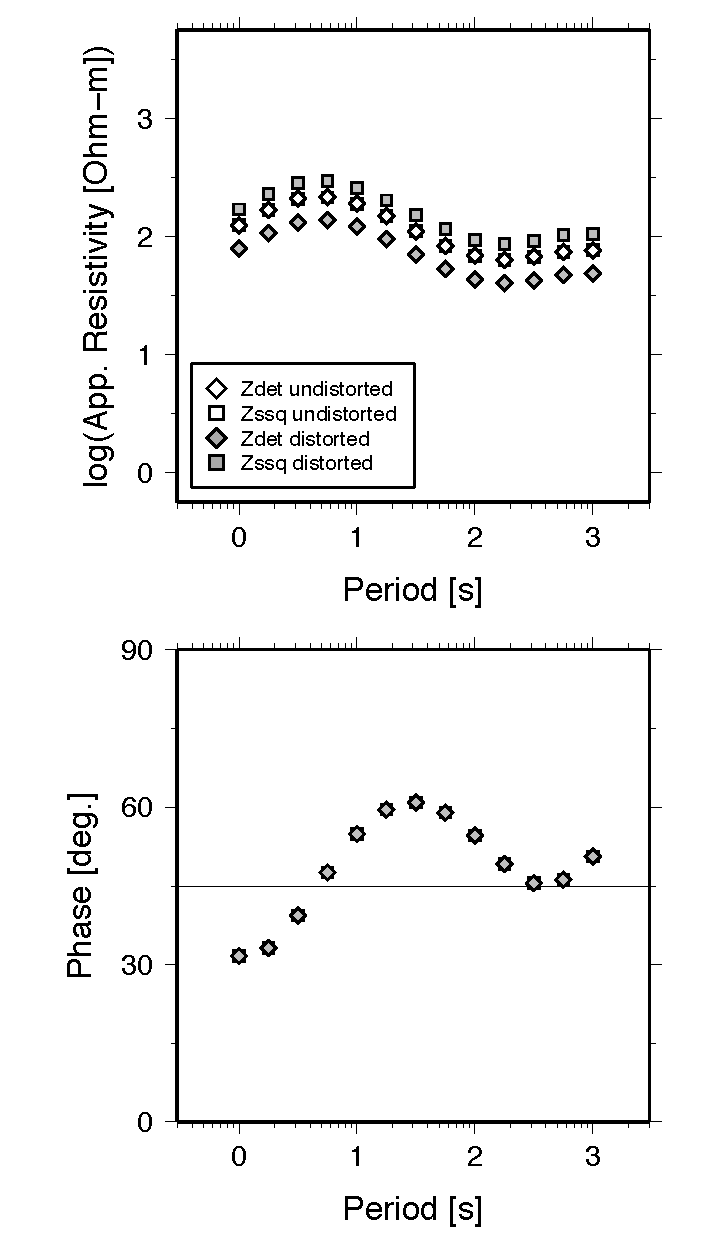
\includegraphics[scale=\plotmtrespscale]{\figdir/lyr11a_syn0203_zinv.pdf}
		\label{fig:resp1d_example_distorted_zinv}
		}
	\caption[Example of distorted 1D MT data and corresponding invariant impedances]{(a) Components of the 1D MT impedance distorted with $(g, t, e, s) = (1.20, 0.11, -0.37, 0.49)$. (b) Corresponding det (diamonds) and ssq (squares) impedances.}
	\label{fig:resp1d_example_distorted}
	\end{figure}
	
%% ==== Figure: Distored 1D response individual all sd3a
\begin{figure}[t]
	\centering
	\subfigure[]{
		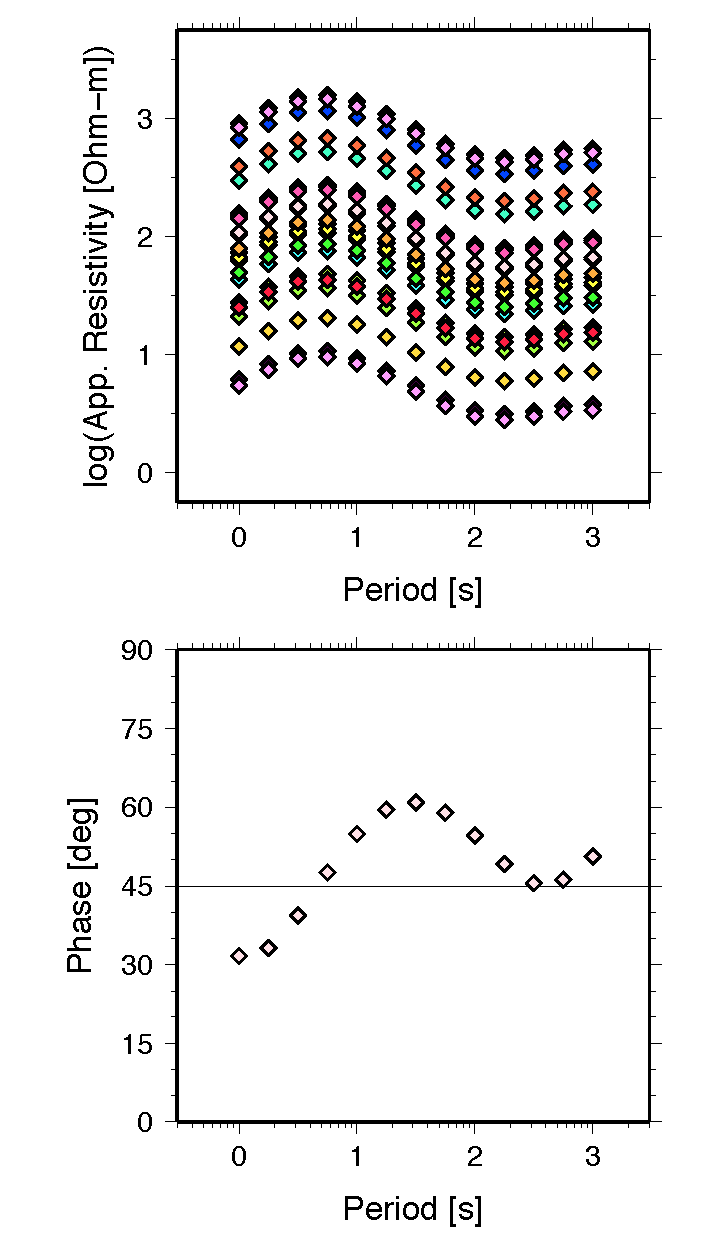
\includegraphics[scale=\plotmtrespscale]{\figdir/lyr11a_n25_d13a_distorted-sd3a-gtes_zinv_det_arsphs.pdf}
		\label{fig:resp1d_individual_all_distorted_sd3a_det}
	}
	\subfigure[]{
		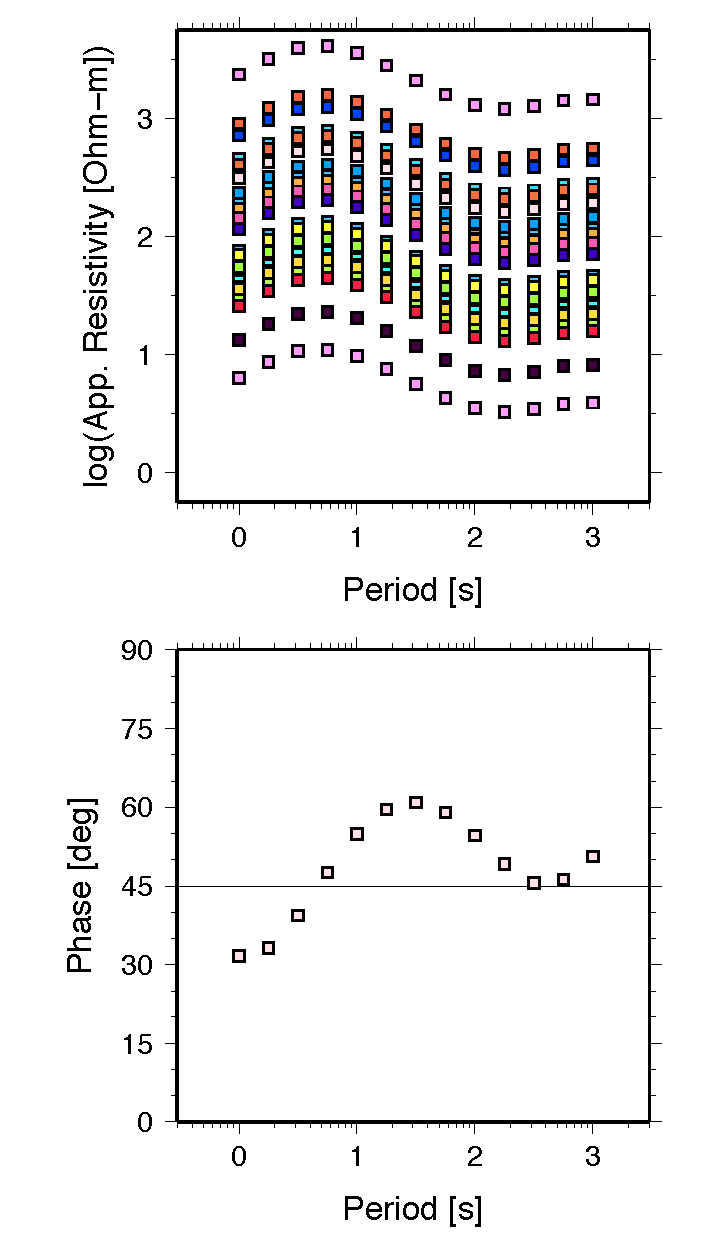
\includegraphics[scale=\plotmtrespscale]{\figdir/lyr11a_n25_d13a_distorted-sd3a-gtes_zinv_ssq_arsphs.pdf}
		\label{fig:resp1d_individual_all_distorted_sd3a_ssq}
	}
	\caption[Example of distorted det and ssq impedances from distorted 1D MT dataset]{Distorted (a) det and (b) ssq impedances from the 1D example, where a set of distortion parameters with an SD of 0.3 was applied. Each station is represented by a different symbol color.}
	\label{fig:resp1d_individual_all_distorted_sd3a}
\end{figure}
%% ==== Figure: Distored 1D response individual average
\begin{figure}[t]
	\centering
	\subfigure[]{
		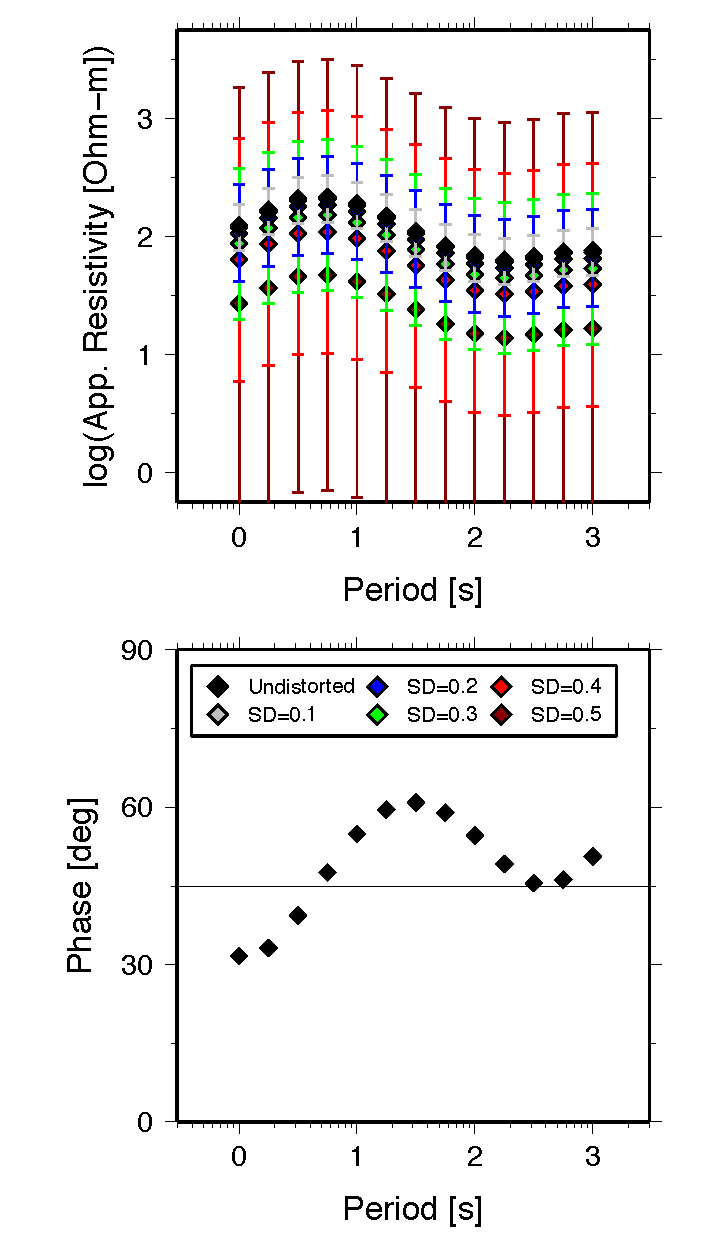
\includegraphics[scale=\plotmtrespscale]{\figdir/lyr11a_d13a_distorted-sdxa_mt_det.pdf}
		\label{fig:resp1d_avg_distorted_det}
	}
	%
	\subfigure[]{
		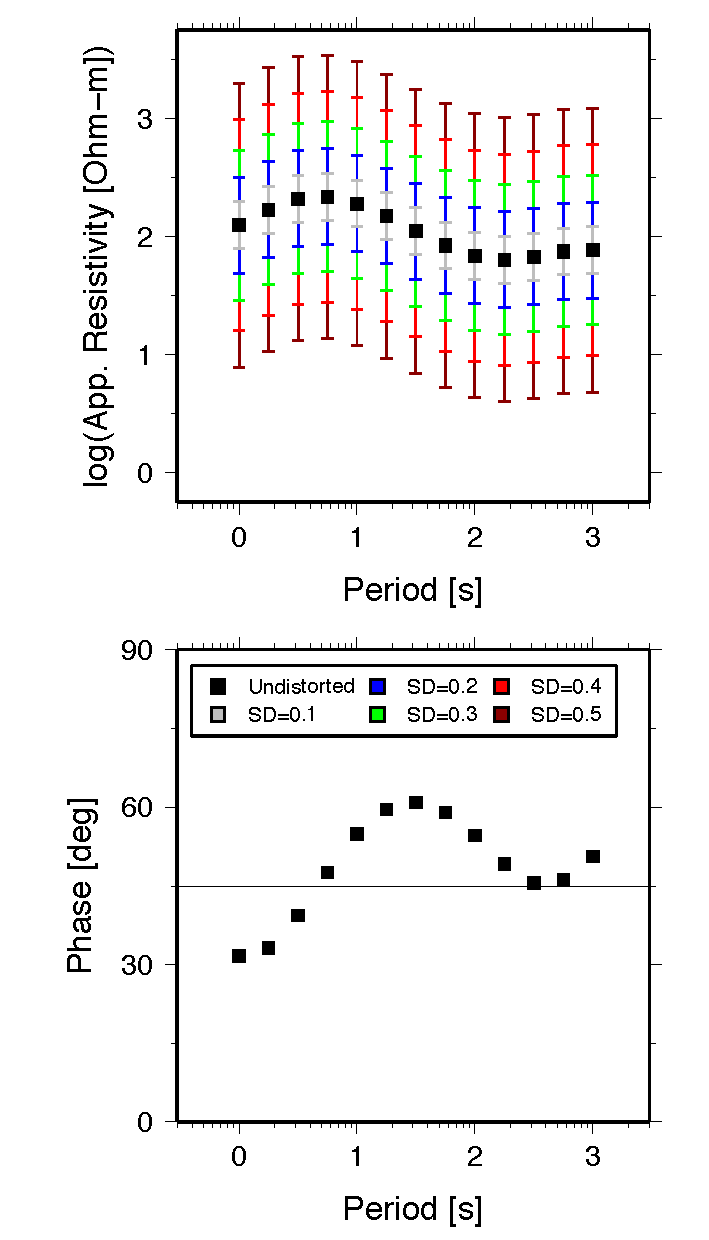
\includegraphics[scale=\plotmtrespscale]{\figdir/lyr11a_d13a_distorted-sdxa_mt_ssq.pdf}
		\label{fig:resp1d_avg_distorted_ssq}
	}
	\caption[Average det and ssq impedances from 1D MT datasets distorted with different galvanic distortion strengths]{Average (a) det and (b) ssq impedances from the 1D datasets distorted with different galvanic distortion strengths.}
	\label{fig:resp1d_avg_distorted}
\end{figure}

%% ==== Results Inverted model
% \red{-- Inverted models --}
 
% \begin{itemize}
%	\item 
	In this work, the Occam 1D inversion \citep{constable1987a} is used to yield the 1D models, in which the second derivative of the conductivity with respect to the depth is penalized. 
	The errors of the apparent resistivity and phase applied in the inversion were fixed at 2.3\% and 0.66$^\circ$, respectively. All inverted models shown in this work fit the data within a root mean square (RMS) error of unity.
%	\item 
	The inverted models from the average det impedances will be less resistive or more conductive than the true structure, particularly when the galvanic distortion is strong.
	On the other hand, the average ssq impedances give models that are very close to the true structure regardless of galvanic distortion strengths.
%	\item 
	From the synthetic tests, when the galvanic distortion is included, the true 1D structure may be missed due to the downward-biased det impedance. The average ssq impedances would be the appropriate candidate to estimate the regional mean 1D conductivity profile.
%\end{itemize}




	

	


%% ==== Individual all inverted
% To show that we should not use the individual distorted data to estimate the regional 1D
%\missingfigure[figwidth=6cm]{Individual all inverted}

%% ==== Figure: Distored 1D response individual sd3a det inverted
%\begin{figure}
%\end{figure}

%% ==== Figure: Distored 1D response average inverted
\begin{figure}[ht]
	\centering
	\subfigure[]{
		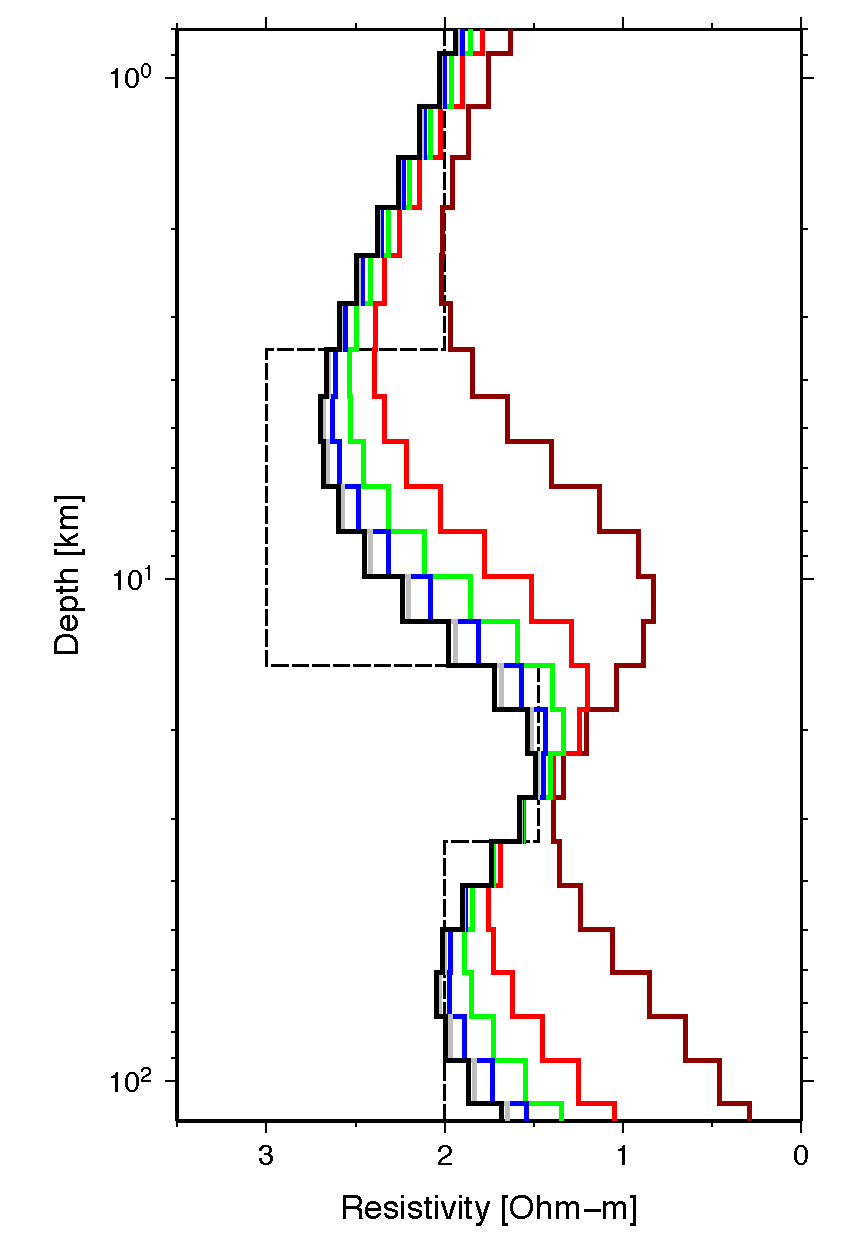
\includegraphics[scale=\plotinvmodelscale]{\figdir/lyr11a_n25_d13a_distorted-sdxa_site_dispse_det_inv1d.pdf}
		\label{fig:resp1d_avg_distorted_model_det}
	}
	\subfigure[]{
		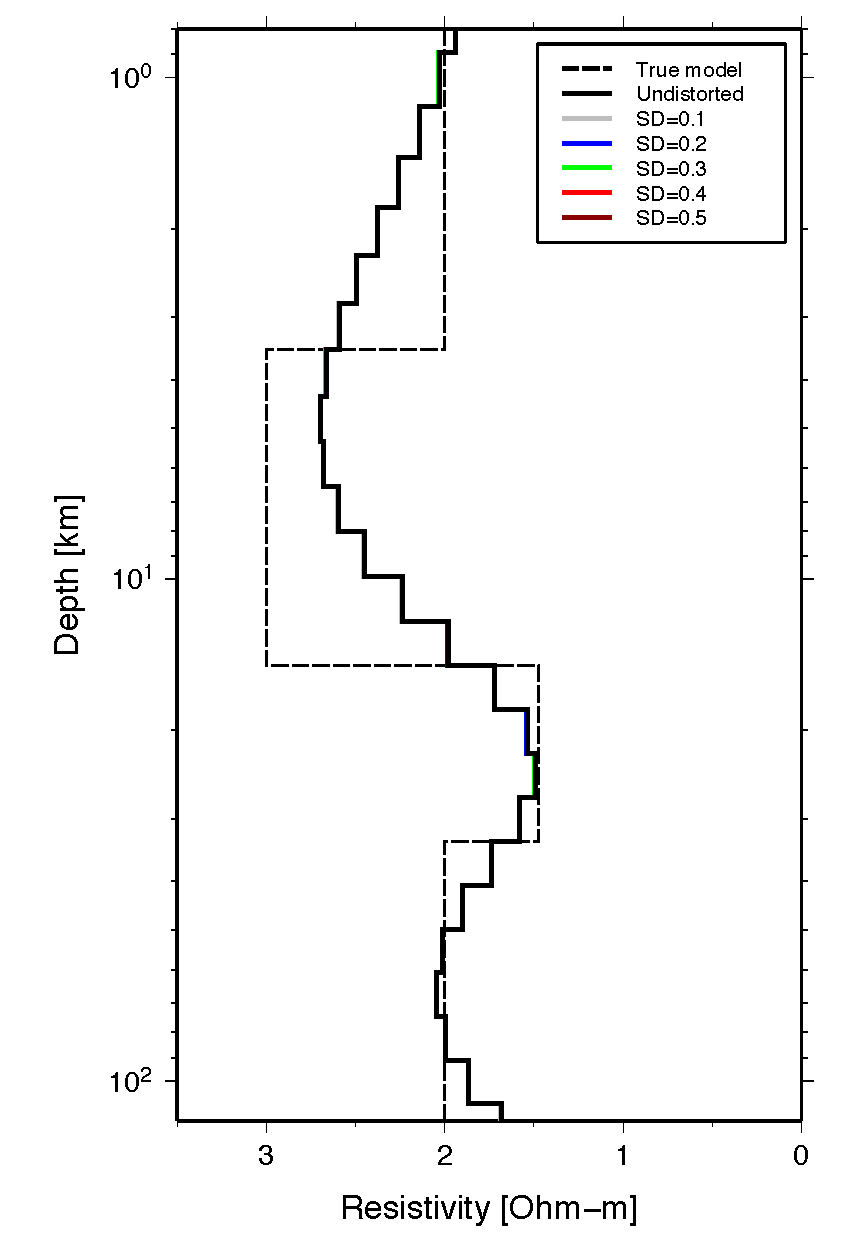
\includegraphics[scale=\plotinvmodelscale]{\figdir/lyr11a_n25_d13a_distorted-sdxa_site_dispse_ssq_inv1d.pdf}
		\label{fig:resp1d_avg_distorted_model_ssq}
	}
	\caption[Inverted models from average det and ssq impedances from distorted 1D datasets]{1D models obtained by inverting the average (a) det and (b) ssq impedances from the distorted 1D datasets (Figure \ref{fig:resp1d_avg_distorted}). The true structure (dashed lines) is also shown for comparison.}
	\label{fig:resp1d_avg_distorted_model}
\end{figure}
